\documentclass[a4paper, landscape]{article}
\usepackage{tikz}
\begin{document}
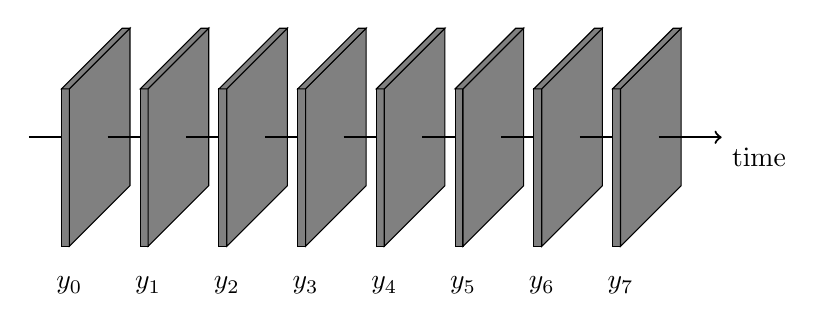
\begin{tikzpicture}
\pgfmathsetmacro{\matrixw}{0.1}
\pgfmathsetmacro{\matrixl}{2}
\pgfmathsetmacro{\vectorw}{0.1}
\iffalse
\foreach \i in {0, 1, 2.5}{
	\draw[black,fill=gray] (\i,0,0) -- ++(-\matrixw,0,0) -- ++(0,-\matrixl,0) -- ++(\matrixw,0,0) -- cycle;
	\draw[black,fill=gray] (\i,0,0) -- ++(0,0,-\matrixl) -- ++(0,-\matrixl,0) -- ++(0,0,\matrixl) -- cycle;
	\draw[black,fill=gray] (\i,0,0) -- ++(-\matrixw,0,0) -- ++(0,0,-\matrixl) -- ++(\matrixw,0,0) -- cycle;
}
\node[draw=none] (ellipsis1) at (1.5,-1, -1) {$\cdots$};
\foreach \i in {0, 1}{
	\node[] at (\i, -2.5) {$y_\i$};
}
\node[] at (2.5, -2.5) {$y_n$};
\draw[thick,->] (2.5 + \matrixw, -1, -1) -- (3.5 - \matrixw, -1, -1) node[anchor=south west] {$\mathcal{L}$}; 

\foreach \i in {0, 1, 2.5}{
	\draw[black,fill=gray, fill opacity=0] (\i + 4.5,0,0) -- ++(-\matrixw,0,0) -- ++(0,-\matrixl,0) -- ++(\matrixw,0,0) -- cycle;
	\draw[black,fill=gray, fill opacity=0] (\i + 4.5,0,0) -- ++(0,0,-\matrixl) -- ++(0,-\matrixl,0) -- ++(0,0,\matrixl) -- cycle;
	\draw[black,fill=gray, fill opacity=0] (\i + 4.5,0,0) -- ++(-\matrixw,0,0) -- ++(0,0,-\matrixl) -- ++(\matrixw,0,0) -- cycle;
	\foreach \c [count=\j] in {red, magenta, yellow, green, cyan, blue} {
		\draw[black,fill=\c] (\i + 4.5,0,\j * 0.4 - 2.4) -- ++(-\matrixw,0,0) -- ++(0,-\matrixl,0) -- ++(\matrixw,0,0) -- cycle;
		\draw[black,fill=\c] (\i + 4.5,0,\j * 0.4 - 2.4) -- ++(0,0,-\vectorw) -- ++(0,-\matrixl,0) -- ++(0,0,\vectorw) -- cycle;
		\draw[black,fill=\c] (\i + 4.5,0,\j * 0.4 - 2.4) -- ++(-\matrixw,0,0) -- ++(0,0,-\vectorw) -- ++(\matrixw,0,0) -- cycle;

	}
}
\node[draw=none] (ellipsis1) at (6.25,-1, -1) {$\cdots$};
\foreach \i in {0, 1}{
	\node[] at (\i + 4.5, -2.5) {$\hat{y_\i}$};
}
\node[] at (7, -2.5) {$\hat{y_n}$};
\draw[thick,->] (7.5 + \matrixw, -1, -1) -- (8.5 - \matrixw, -1, -1) node[anchor=south west] {}; 

\foreach \i in {0, 0.5, 2}{
	\foreach \c [count=\j] in {red, magenta, yellow, green, cyan, blue} {
		\draw[black,fill=\c] (\i + 9,\j * 0.4 - 2.4,0) -- ++(-\vectorw,0,0) -- ++(0,-\vectorw,0) -- ++(\vectorw,0,0) -- cycle;
		\draw[black,fill=\c] (\i + 9,\j * 0.4 - 2.4,0) -- ++(0,0,-\matrixl) -- ++(0,-\vectorw,0) -- ++(0,0,\matrixl) -- cycle;
		\draw[black,fill=\c] (\i + 9,\j * 0.4 - 2.4,0) -- ++(-\vectorw,0,0) -- ++(0,0,-\matrixl) -- ++(\vectorw,0,0) -- cycle;
	}
}
\foreach \c [count=\j] in {red, magenta, yellow, green, cyan, blue} {
	\draw[thick,->] (11,\j * 0.4 - 2.4,-1) -- (12,\j * 0.4 - 2.4,-1) node[anchor=south west] {VAR}; 
	\draw[thick,->] (13,\j * 0.4 - 2.4,-1) -- (13.5,\j * 0.4 - 2.4,-1) node[anchor=south west] {}; 
}
\node[draw=none] (ellipsis1) at (10.25,-1, -1) {$\cdots$};

\foreach \i in {0, 0.5, 2}{
	\foreach \c [count=\j] in {red, magenta, yellow, green, cyan, blue} {
		\draw[black,fill=\c] (\i + 13.5,\j * 0.4 - 2.4,0) -- ++(-\vectorw,0,0) -- ++(0,-\vectorw,0) -- ++(\vectorw,0,0) -- cycle;
		\draw[black,fill=\c] (\i + 13.5,\j * 0.4 - 2.4,0) -- ++(0,0,-\matrixl) -- ++(0,-\vectorw,0) -- ++(0,0,\matrixl) -- cycle;
		\draw[black,fill=\c] (\i + 13.5,\j * 0.4 - 2.4,0) -- ++(-\vectorw,0,0) -- ++(0,0,-\matrixl) -- ++(\vectorw,0,0) -- cycle;
	}
}
\node[draw=none] (ellipsis1) at (14.75,-1, -1) {$\cdots$};
\fi

\foreach \i in {0, 1, 2, 3, 4, 5, 6, 7}{
	\draw[thick,->] (-1 + \i + \matrixw, -1, -1) -- (\i - \matrixw, -1, -1);
	\draw[black,fill=gray] (\i,0,0) -- ++(-\matrixw,0,0) -- ++(0,-\matrixl,0) -- ++(\matrixw,0,0) -- cycle;
	\draw[black,fill=gray] (\i,0,0) -- ++(0,0,-\matrixl) -- ++(0,-\matrixl,0) -- ++(0,0,\matrixl) -- cycle;
	\draw[black,fill=gray] (\i,0,0) -- ++(-\matrixw,0,0) -- ++(0,0,-\matrixl) -- ++(\matrixw,0,0) -- cycle;
	\node[] at (\i, -2.5) {$y_\i$};
}
\draw[thick,->] (7 + \matrixw, -1, -1) -- (8 - \matrixw, -1, -1) node[anchor=north west] {time}; 

\end{tikzpicture}
\end{document}